\documentclass{beamer}

\mode<presentation>

\usepackage{dirtree}
\usepackage{ifthen}
\usepackage[utf8]{inputenc}
\usepackage{listings}
\usepackage{minted}
\usepackage{xcolor}
\usepackage{xifthen}

\setbeamertemplate{footline}[frame number]
\usetheme{Singapore}
\usecolortheme{seagull}
\newenvironment{Frame}{\begin{frame}[containsverbatim]{\subsecname}}{\end{frame}}
\newenvironment{FrameTP}{\begin{frame}[containsverbatim]{\secname}}{\end{frame}}

\lstdefinestyle{lst_base_style}{
    language=C,
    numbers=left,
    basicstyle=\ttfamily,
    keywordstyle=\color{blue}\ttfamily,
    identifierstyle=\color{brown}\ttfamily,
    stringstyle=\color{teal}\ttfamily,
    commentstyle=\color{gray}\ttfamily
}
\lstset{style=lst_base_style, texcl=true}
\newcommand{\PrintSnippet}[5]{
    \ifthenelse{\isempty{#5}}
    {
        \lstinputlisting[title=#2, language=#1]{#3}
    }
    {
        \lstinputlisting[title=#2,
            firstline=#4, lastline=#5, firstnumber=#4
        ]{#3}
    }
}
\newcommand{\ProjectView}[2]{
    \begin{columns}[T]
        \column{\dimexpr \paperwidth-0.8\textwidth}
        #1
        \column{0.6\textwidth}   
        #2
    \end{columns}
}

\title{Introduction au kit de développement logiciel Pico SDK}

\author{
   
\includegraphics[height=3cm]{Raspberry_Pi.png}
}

\begin{document}

\begin{frame}
    \maketitle
\end{frame}

\begin{frame}
    \small
    \tableofcontents
\end{frame}

\section{Variables et listes}

\subsection{Un système similaire à celui du langage Bash}

\begin{Frame}
    \begin{itemize}
        \item Aucun typage (ce qui est différent du typage statique en C et du typage dynamique en Python)
        \item Variables définies par défaut
        \item Lecture des variables par expansion, par exemple en Bash
        \begin{minted}{bash}
MY_VAR=Hello
echo MY_VAR  # Affiche 'MY_VAR'
echo $MY_VAR # Afficher 'Hello'
        \end{minted}
    \end{itemize}
\end{Frame}

\begin{Frame}
    \begin{minted}{cmake}
set(EXECUTABLE_NAME MyExecutable)
set(EXECUTABLE_SOURCES "")
list(APPEND EXECUTABLE_SOURCES main.c)
list(APPEND EXECUTABLE_SOURCES aux.c)
add_executable(${EXECUTABLE_NAME} ${EXECUTABLE_SOURCES})
    \end{minted}
\end{Frame}

\subsection{La commande \texttt{set} pour définir ou modifier une variable}

\begin{Frame}
    \small
    \begin{minted}{cmake}
set(<variable> <value>... [PARENT_SCOPE])
set(<variable> <value>... CACHE <type> <docstring> [FORCE])
set(ENV{<variable>} [<value>])
    \end{minted}
\end{Frame}

\subsection{La visibilité des variables}

\newcommand{\PrintCMakeSnippet}[2]{
    \begin{center}   
        #1
        \vspace{0.5em}
        \hline
    \end{center}
    \texttt{#2}
}

\begin{Frame}
    \ProjectView{
        \dirtree{%
            .1 project/.
                .2 CMakeLists.txt.
                .2 src/.
                    .3 CMakeLists.txt.
        }
    }{
        \PrintCMakeSnippet{CMakeLists.txt}{%
            add\_subdirectory(src)
            message(WARNING \$\{MY\_VAR\})
        }
        \PrintCMakeSnippet{src/CMakeLists.txt}{%
            set(MY\_VAR "Hello")%
        }
    }
\end{Frame}

\begin{Frame}
    \begin{minted}{bash}
$ cmake -B build
CMake Warning at CMakeLists.txt:5 (message):


-- Configuring done
-- Generating done
-- Build files have been written to: ...       
    \end{minted}
\end{Frame}

\begin{Frame}
    \ProjectView{
        \dirtree{%
            .1 project/.
                .2 CMakeLists.txt.
                .2 src/.
                    .3 CMakeLists.txt.
        }
    }{
        \PrintCMakeSnippet{CMakeLists.txt}{%
            add\_subdirectory(src)
            message(WARNING \$\{MY\_VAR\})
        }
        \PrintCMakeSnippet{src/CMakeLists.txt}{%
            set(MY\_VAR "Hello" PARENT\_SCOPE)%
        }
    }
\end{Frame}

\begin{Frame}
    \begin{minted}{bash}
$ cmake -B build
CMake Warning at CMakeLists.txt:5 (message):
Hello

-- Configuring done
-- Generating done
-- Build files have been written to: ...       
    \end{minted}
\end{Frame}

\subsection{La commande \texttt{list} pour traiter une variable comme une liste}

\begin{Frame}
    \tiny
    \begin{minted}{cmake}
Reading
  list(LENGTH <list> <out-var>)
  list(GET <list> <element index> [<index> ...] <out-var>)
  list(JOIN <list> <glue> <out-var>)
  list(SUBLIST <list> <begin> <length> <out-var>)

Search
  list(FIND <list> <value> <out-var>)

Modification
  list(APPEND <list> [<element>...])
  list(FILTER <list> {INCLUDE | EXCLUDE} REGEX <regex>)
  list(INSERT <list> <index> [<element>...])
  list(POP_BACK <list> [<out-var>...])
  list(POP_FRONT <list> [<out-var>...])
  list(PREPEND <list> [<element>...])
  list(REMOVE_ITEM <list> <value>...)
  list(REMOVE_AT <list> <index>...)
  list(REMOVE_DUPLICATES <list>)
  list(TRANSFORM <list> <ACTION> [...])

Ordering
  list(REVERSE <list>)
  list(SORT <list> [...])
    \end{minted}
\end{Frame}

\subsection{Déclarer une liste}

\begin{Frame}
    \begin{minted}{cmake}
set(MY_LIST "Hello" "There !" "Hello There !")
message(${MY_LIST})
message("${MY_LIST}")

set(MY_LIST Hello There ! Hello There !)
message(${MY_LIST})
message("${MY_LIST}")
    \end{minted}
\end{Frame}

\begin{Frame}
    \begin{minted}{bash}
$ cmake -B build
HelloThere !Hello There !
Hello;There !;Hello There !
HelloThere!HelloThere!
Hello;There;!;Hello;There;!
-- Configuring done
-- Generating done
-- Build files have been written to: ...
    \end{minted}
\end{Frame}

\subsection{La sous-commande \texttt{APPEND} de \texttt{list}}

\begin{Frame}
    \begin{minted}{cmake}
set(MY_LIST "Hello" "There !" "Hello There !")
list(APPEND MY_LIST "Hi !")
message(${MY_LIST})
message("${MY_LIST}")
    \end{minted}
\end{Frame}

\begin{Frame}
    \begin{minted}{bash}
$ cmake -B build
HelloThere !Hello There !Hi !
Hello;There !;Hello There !;Hi !
-- Configuring done
-- Generating done
-- Build files have been written to: ...
    \end{minted}
\end{Frame}

\section{Modules et fonctions}

\subsection{La variable spéciale \texttt{CMAKE\_MODULE\_PATH}}

\begin{Frame}
    \ProjectView{
        \dirtree{%
            .1 project/.
                .2 CMakeLists.txt.
                .2 tool/.
                    .3 MyModule.cmake.
        }
    }{
        \PrintCMakeSnippet{
            CMakeLists.txt
        }{
            include(MyModule)
        }
    }
\end{Frame}

\begin{Frame}
    \begin{minted}{bash}
$ cmake -B build
CMake Error at CMakeLists.txt:5 (include):
  include could not find requested file:

    MyModule


-- Configuring incomplete, errors occurred!
    \end{minted}
\end{Frame}

\begin{Frame}
    \ProjectView{
        \dirtree{%
            .1 project/.
                .2 CMakeLists.txt.
                .2 tool/.
                    .3 MyModule.cmake.
        }
    }{
        \PrintCMakeSnippet{
            CMakeLists.txt
        }{%
            list(APPEND
                CMAKE\_MODULE\_PATH
                \$\{PROJECT\_SOURCE\_DIR\}/tool)
            include(MyModule)
        }
    }
\end{Frame}

\subsection{Définir une fonction}

\begin{Frame}
    \begin{minted}{cmake}
        function(my_function A B C)
            message("${A} ${B} ${C}")
        endfunction()

        my_function("Hello" "there" "!")
    \end{minted}
\end{Frame}

\begin{Frame}
    \begin{minted}{bash}
$ cmake -B build
Hello there !
-- Configuring done
-- Generating done
-- Build files have been written to: ...
    \end{minted}
\end{Frame}

\section{TP : Créer un module}

\begin{FrameTP}
    Écrivez un module qui défini une fonction de votre choix.
    
    Pour tester, le module, écrivez un \verb|CMakeLists.txt| qui inclut le module et appelle la fonction.
\end{FrameTP}

\section{Pico SDK}

\subsection{Pico SDK}

\begin{Frame}
    \begin{itemize}
        \item Le SDK se présente comme \textbf{un projet CMake}
        \item Le dépôt SDK se trouve sur GitHub (possibilité d'utiliser FetchContent)
        \item Le SDK fourni \textbf{des modules}, \textbf{des fonctions CMake} (qui se trouvent dans le dossier \texttt{external/} du dépôt) et \textbf{des bibliothèques} (à linker avec vos exécutables)
        \item La difficulté est \textbf{d'inclure le SDK dans votre projet CMake}
    \end{itemize}
\end{Frame}

\subsection{Initialisation du SDK}

\begin{Frame}
    \small
    \begin{minted}{cmake}
...

FetchContent_Declare(pico-sdk
    GIT_REPOSITORY https://github.com/raspberrypi/pico-sdk
    GIT_SUBMODULES_RECURSE OFF)

...

include(pico_sdk_import)

...

project(TechTheTaste_LowLevel LANGUAGES C CXX ASM)
    \end{minted}
\end{Frame}

\subsection{Activer et désactiver des fonctionnalités du SDK}

\begin{Frame}
    \begin{minted}{cmake}
# `printf()` écrit sur la liaison USB
pico_enable_stdio_usb(MyExecutable ON)

# `printf()` écrit sur la liaison UART
pico_enable_stdio_uart(MyExecutable ON)
    \end{minted}
\end{Frame}

\subsection{Une étape supplémentaire après la production de l'exécutable}

\begin{Frame}
    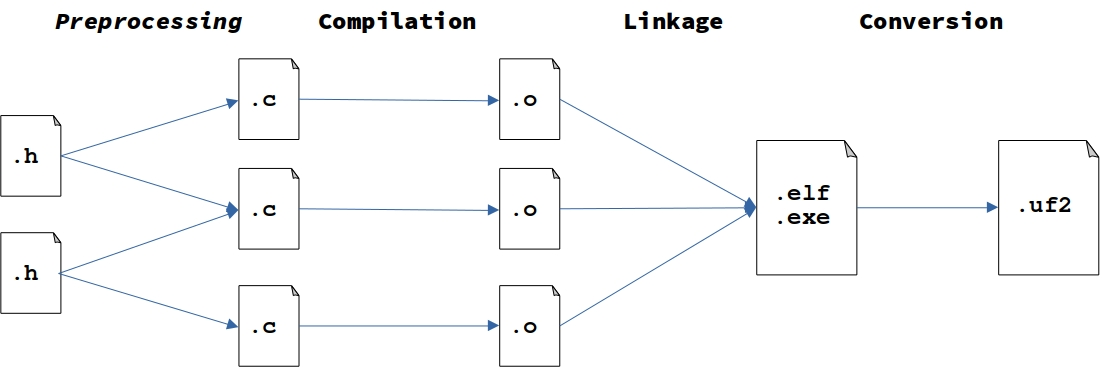
\includegraphics[width=\textwidth]{compilation_steps_uf2.jpg}
    \begin{minted}{cmake}
pico_add_extra_outputs(MyExecutable)
    \end{minted}
\end{Frame}

\section{TP: Projet CMake + Pico SDK}

\begin{FrameTP}
    Ce TP est à réaliser en groupe de 2 ou 3 personnes.
    \begin{itemize}
        \item Créez un dépôt GitHub pour le TP
        \item Initialiser le dépôt avec l'arborescence suivante
        \vspace{-1em}
        \dirtree{%
            .1 .
                .2 CMakeLists.txt.
                .2 log/.
                    .3 CMakeLists.txt.
                .2 init/.
                    .3 CMakeLists.txt.
        }
        Les fichiers doivent être \textbf{vides}
        \item Télécharger le dépôt sur l'ordinateur de chaque membre puis créer une branche par membre
    \end{itemize}
\end{FrameTP}

\begin{FrameTP} 
    Répartissez les tâches suivantes entre les membres du groupes :
    \begin{itemize}
        \item Dans le dossier \texttt{init/}, écrivez une fonction qui initialise la liaison USB
        \item Dans le dossier \texttt{log/}, écrivez une fonction qui permet de d'écrire sur la liaison USB
        \item A la racine du projet, écrivez une fonction \verb|main| qui utilise les deux fonctions précédentes
    \end{itemize}
    Une contrainte supplémentaire est ajoutée : \textbf{vous ne devez pas écrire en dehors du répertoire qui vous est réservé}. Vous ne devez pas non plus faire de \textit{commits} en dehors de votre branche. En revanche, vous avez le droit de fusionner les branches avec la branche \texttt{main}
\end{FrameTP}

\end{document}
